\section{Durchführung}

Eine Skizze der Messapparatur ist in Abbildung \ref{abb:3} dargestellt. Zur Erzeugung
eines parallelen Lichtbündels wird ein He-Ne-Laser verwendet.

\begin{figure}[H]
  \centering
  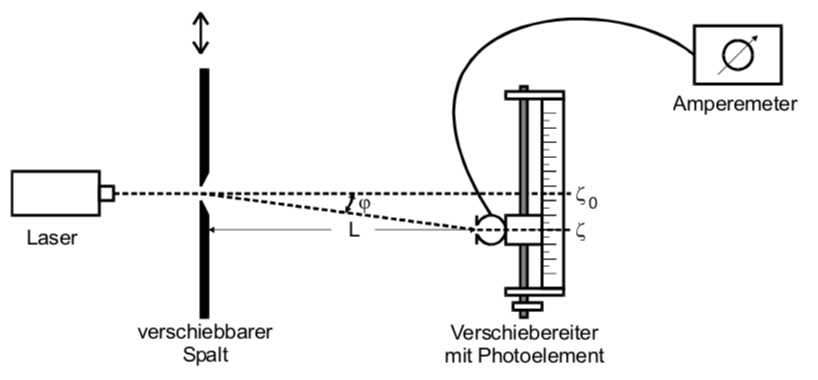
\includegraphics[width=\textwidth]{content/Versuchsaufbau.png}
  \caption{Versuchsaufbau zur Ausmessung der Beugungsfigur \cite{1}.}
  \label{abb:3}
\end{figure}

Der Detektor befindet sich etwa $100-120 \si{\centi\meter}$ hinter dem Spalt.
Dieser Detektor ist auf einem Verschiebereiter, mit dem der Detektor parallel zum
Spalt verschoben werden kann.
Bevor mit der Messung begonnen werden kann wird mit dem Detektor eine Messung der
Lichtintensität $I_{\text{du}}$ mit abgedecktem Laser durchgeführt. Dieser Wert muss
in der Auswertung immer von den Messwerten abgezogen werden.

Daraufhin wird zunächst die Beugungsfigur von zwei verschiedenen Einzelspalten
ausgemessen und zuletzt eine Beugungsfigur von einem Doppelspalt.

Um aus der Detektorstellung $\xi$ den Winkel $\varphi$ zu bestimmen wird folgende
Gleichung verwendet

\begin{equation}
  \varphi \approx \tan(\varphi) = \frac{\xi - \xi_0}{L}.
  \label{eq:3}
\end{equation}

Dabei ist $L$ der Abstand zwischen Detektor und Spalt und $\xi_0$ ist die Detektorstellung
des ungebeugten Strahles.
